% Options for packages loaded elsewhere
\PassOptionsToPackage{unicode}{hyperref}
\PassOptionsToPackage{hyphens}{url}
%
\documentclass[
]{article}
\usepackage{amsmath,amssymb}
\usepackage{lmodern}
\usepackage{ifxetex,ifluatex}
\ifnum 0\ifxetex 1\fi\ifluatex 1\fi=0 % if pdftex
  \usepackage[T1]{fontenc}
  \usepackage[utf8]{inputenc}
  \usepackage{textcomp} % provide euro and other symbols
\else % if luatex or xetex
  \usepackage{unicode-math}
  \defaultfontfeatures{Scale=MatchLowercase}
  \defaultfontfeatures[\rmfamily]{Ligatures=TeX,Scale=1}
\fi
% Use upquote if available, for straight quotes in verbatim environments
\IfFileExists{upquote.sty}{\usepackage{upquote}}{}
\IfFileExists{microtype.sty}{% use microtype if available
  \usepackage[]{microtype}
  \UseMicrotypeSet[protrusion]{basicmath} % disable protrusion for tt fonts
}{}
\makeatletter
\@ifundefined{KOMAClassName}{% if non-KOMA class
  \IfFileExists{parskip.sty}{%
    \usepackage{parskip}
  }{% else
    \setlength{\parindent}{0pt}
    \setlength{\parskip}{6pt plus 2pt minus 1pt}}
}{% if KOMA class
  \KOMAoptions{parskip=half}}
\makeatother
\usepackage{xcolor}
\IfFileExists{xurl.sty}{\usepackage{xurl}}{} % add URL line breaks if available
\IfFileExists{bookmark.sty}{\usepackage{bookmark}}{\usepackage{hyperref}}
\hypersetup{
  pdftitle={Compulsory exercise 1: Group 16},
  pdfauthor={Weicheng Hua, Emil Johannese Haugstvedt, Torbjørn Baadsvik},
  hidelinks,
  pdfcreator={LaTeX via pandoc}}
\urlstyle{same} % disable monospaced font for URLs
\usepackage[margin=1in]{geometry}
\usepackage{color}
\usepackage{fancyvrb}
\newcommand{\VerbBar}{|}
\newcommand{\VERB}{\Verb[commandchars=\\\{\}]}
\DefineVerbatimEnvironment{Highlighting}{Verbatim}{commandchars=\\\{\}}
% Add ',fontsize=\small' for more characters per line
\usepackage{framed}
\definecolor{shadecolor}{RGB}{248,248,248}
\newenvironment{Shaded}{\begin{snugshade}}{\end{snugshade}}
\newcommand{\AlertTok}[1]{\textcolor[rgb]{0.94,0.16,0.16}{#1}}
\newcommand{\AnnotationTok}[1]{\textcolor[rgb]{0.56,0.35,0.01}{\textbf{\textit{#1}}}}
\newcommand{\AttributeTok}[1]{\textcolor[rgb]{0.77,0.63,0.00}{#1}}
\newcommand{\BaseNTok}[1]{\textcolor[rgb]{0.00,0.00,0.81}{#1}}
\newcommand{\BuiltInTok}[1]{#1}
\newcommand{\CharTok}[1]{\textcolor[rgb]{0.31,0.60,0.02}{#1}}
\newcommand{\CommentTok}[1]{\textcolor[rgb]{0.56,0.35,0.01}{\textit{#1}}}
\newcommand{\CommentVarTok}[1]{\textcolor[rgb]{0.56,0.35,0.01}{\textbf{\textit{#1}}}}
\newcommand{\ConstantTok}[1]{\textcolor[rgb]{0.00,0.00,0.00}{#1}}
\newcommand{\ControlFlowTok}[1]{\textcolor[rgb]{0.13,0.29,0.53}{\textbf{#1}}}
\newcommand{\DataTypeTok}[1]{\textcolor[rgb]{0.13,0.29,0.53}{#1}}
\newcommand{\DecValTok}[1]{\textcolor[rgb]{0.00,0.00,0.81}{#1}}
\newcommand{\DocumentationTok}[1]{\textcolor[rgb]{0.56,0.35,0.01}{\textbf{\textit{#1}}}}
\newcommand{\ErrorTok}[1]{\textcolor[rgb]{0.64,0.00,0.00}{\textbf{#1}}}
\newcommand{\ExtensionTok}[1]{#1}
\newcommand{\FloatTok}[1]{\textcolor[rgb]{0.00,0.00,0.81}{#1}}
\newcommand{\FunctionTok}[1]{\textcolor[rgb]{0.00,0.00,0.00}{#1}}
\newcommand{\ImportTok}[1]{#1}
\newcommand{\InformationTok}[1]{\textcolor[rgb]{0.56,0.35,0.01}{\textbf{\textit{#1}}}}
\newcommand{\KeywordTok}[1]{\textcolor[rgb]{0.13,0.29,0.53}{\textbf{#1}}}
\newcommand{\NormalTok}[1]{#1}
\newcommand{\OperatorTok}[1]{\textcolor[rgb]{0.81,0.36,0.00}{\textbf{#1}}}
\newcommand{\OtherTok}[1]{\textcolor[rgb]{0.56,0.35,0.01}{#1}}
\newcommand{\PreprocessorTok}[1]{\textcolor[rgb]{0.56,0.35,0.01}{\textit{#1}}}
\newcommand{\RegionMarkerTok}[1]{#1}
\newcommand{\SpecialCharTok}[1]{\textcolor[rgb]{0.00,0.00,0.00}{#1}}
\newcommand{\SpecialStringTok}[1]{\textcolor[rgb]{0.31,0.60,0.02}{#1}}
\newcommand{\StringTok}[1]{\textcolor[rgb]{0.31,0.60,0.02}{#1}}
\newcommand{\VariableTok}[1]{\textcolor[rgb]{0.00,0.00,0.00}{#1}}
\newcommand{\VerbatimStringTok}[1]{\textcolor[rgb]{0.31,0.60,0.02}{#1}}
\newcommand{\WarningTok}[1]{\textcolor[rgb]{0.56,0.35,0.01}{\textbf{\textit{#1}}}}
\usepackage{graphicx}
\makeatletter
\def\maxwidth{\ifdim\Gin@nat@width>\linewidth\linewidth\else\Gin@nat@width\fi}
\def\maxheight{\ifdim\Gin@nat@height>\textheight\textheight\else\Gin@nat@height\fi}
\makeatother
% Scale images if necessary, so that they will not overflow the page
% margins by default, and it is still possible to overwrite the defaults
% using explicit options in \includegraphics[width, height, ...]{}
\setkeys{Gin}{width=\maxwidth,height=\maxheight,keepaspectratio}
% Set default figure placement to htbp
\makeatletter
\def\fps@figure{htbp}
\makeatother
\setlength{\emergencystretch}{3em} % prevent overfull lines
\providecommand{\tightlist}{%
  \setlength{\itemsep}{0pt}\setlength{\parskip}{0pt}}
\setcounter{secnumdepth}{-\maxdimen} % remove section numbering
\ifluatex
  \usepackage{selnolig}  % disable illegal ligatures
\fi

\title{Compulsory exercise 1: Group 16}
\usepackage{etoolbox}
\makeatletter
\providecommand{\subtitle}[1]{% add subtitle to \maketitle
  \apptocmd{\@title}{\par {\large #1 \par}}{}{}
}
\makeatother
\subtitle{TMA4268 Statistical Learning V2022}
\author{Weicheng Hua, Emil Johannese Haugstvedt, Torbjørn Baadsvik}
\date{20 February, 2022}

\begin{document}
\maketitle

\hypertarget{problem-1}{%
\section{Problem 1}\label{problem-1}}

\hypertarget{a}{%
\subsection{a)}\label{a}}

The expected MSE on the test set is given by: \[\begin{aligned}
  E[(y_0 - \hat{f}(x_0))^2] &= 
  E[(f(x_0) - \hat{f}(x_0) + \epsilon)^2] \\
  &= E[(f(x_0) - \hat{f}(x_0))^2] + 2E[\epsilon(f(x_0) - \hat{f}(x_0))] + E[\epsilon^2] \\
  &= E[f(x_0)^2 - 2f(x_0)\hat{f}(x_0)] + E[\hat{f}(x_0)^2] + E[\epsilon^2]\\
  &= E[f(x_0)^2 - 2f(x_0)\hat{f}(x_0) + \hat{f}(x_0)^2] 
  + ( E[\hat{f}(x_0)^2] - E[\hat{f}(x_0)]^2) + E[\epsilon^2] \\
  &= E[(f(x_0) - \hat{f}(x_0))^2] + ( E[\hat{f}(x_0)^2] - E[\hat{f}(x_0)]^2) + E[\epsilon^2]\\
  &= E[(f(x_0) - \hat{f}(x_0))^2] + Var[\hat{f}(x_0)] + Var[\epsilon]\\
  &= \text{Squared bias} + \text{Variance of prediction} + \text{Irreducible error}\\ 
\end{aligned}\]

\hypertarget{b}{%
\subsection{b)}\label{b}}

The squared bias term represents the expected squared deviation between
the prediction of the ``true'' model and the prediction of the fitted
model. The variance of prediction term represents the degree to which
the prediction of the fitted model can vary depending on the input.
Higher variance of prediction means the model can adapt it's prediction
to input data to a greater extent than a simpler model, implying that
the model is more flexible. However, the increased ``adaptability'' may
be unwanted if it leads to overfitting.

\hypertarget{c}{%
\subsection{c)}\label{c}}

\[\begin{matrix}
i & ii & iii & iv\\ 
\hline\\
TRUE & FALSE & TRUE & FALSE\\
\end{matrix}\]

\hypertarget{d}{%
\subsection{d)}\label{d}}

\[\begin{matrix}
i & ii & iii & iv\\ 
\hline\\
TRUE & FALSE & TRUE & FALSE\\
\end{matrix}\]

\hypertarget{e}{%
\subsection{e)}\label{e}}

\begin{Shaded}
\begin{Highlighting}[]
\FunctionTok{library}\NormalTok{(matrixcalc)}
\NormalTok{mat }\OtherTok{\textless{}{-}} \FunctionTok{cbind}\NormalTok{(}\FunctionTok{c}\NormalTok{(}\DecValTok{50}\NormalTok{, }\DecValTok{33}\NormalTok{, }\DecValTok{18}\NormalTok{), }\FunctionTok{c}\NormalTok{(}\DecValTok{33}\NormalTok{, }\DecValTok{38}\NormalTok{, }\SpecialCharTok{{-}}\DecValTok{10}\NormalTok{), }\FunctionTok{c}\NormalTok{(}\DecValTok{18}\NormalTok{, }\SpecialCharTok{{-}}\DecValTok{10}\NormalTok{, }\DecValTok{72}\NormalTok{))}
\FunctionTok{is.positive.semi.definite}\NormalTok{(mat)}
\end{Highlighting}
\end{Shaded}

\begin{verbatim}
## [1] TRUE
\end{verbatim}

Answer: iii) 0.76

\hypertarget{problem-2}{%
\section{Problem 2}\label{problem-2}}

Here is a code chunk:

\begin{Shaded}
\begin{Highlighting}[]
\FunctionTok{library}\NormalTok{(palmerpenguins) }\CommentTok{\# Contains the data set "penguins".}
\FunctionTok{data}\NormalTok{(penguins)}
\FunctionTok{head}\NormalTok{(penguins)}
\end{Highlighting}
\end{Shaded}

\begin{verbatim}
## # A tibble: 6 x 8
##   species island bill_length_mm bill_depth_mm flipper_length_~ body_mass_g sex  
##   <fct>   <fct>           <dbl>         <dbl>            <int>       <int> <fct>
## 1 Adelie  Torge~           39.1          18.7              181        3750 male 
## 2 Adelie  Torge~           39.5          17.4              186        3800 fema~
## 3 Adelie  Torge~           40.3          18                195        3250 fema~
## 4 Adelie  Torge~           NA            NA                 NA          NA <NA> 
## 5 Adelie  Torge~           36.7          19.3              193        3450 fema~
## 6 Adelie  Torge~           39.3          20.6              190        3650 male 
## # ... with 1 more variable: year <int>
\end{verbatim}

\hypertarget{a-1}{%
\subsection{a)}\label{a-1}}

\hypertarget{b-1}{%
\subsection{b)}\label{b-1}}

\hypertarget{c-1}{%
\subsection{c)}\label{c-1}}

\hypertarget{problem-3}{%
\section{Problem 3}\label{problem-3}}

Load and prepare data the problem 3

\begin{Shaded}
\begin{Highlighting}[]
\CommentTok{\# Load libraries}
\FunctionTok{library}\NormalTok{(tidyverse)}
\FunctionTok{library}\NormalTok{(class)}
\FunctionTok{library}\NormalTok{(MASS)}
\FunctionTok{library}\NormalTok{(palmerpenguins)}
\FunctionTok{library}\NormalTok{(dplyr)}
\FunctionTok{library}\NormalTok{(caret)}
\FunctionTok{library}\NormalTok{(pROC)}

\CommentTok{\# Load penguins data}
\NormalTok{Penguins }\OtherTok{\textless{}{-}}\NormalTok{ penguins}

\CommentTok{\# Add binary variable: if adelie}
\NormalTok{Penguins}\SpecialCharTok{$}\NormalTok{adelie }\OtherTok{\textless{}{-}} \FunctionTok{ifelse}\NormalTok{(Penguins}\SpecialCharTok{$}\NormalTok{species }\SpecialCharTok{==} \StringTok{"Adelie"}\NormalTok{, }\DecValTok{1}\NormalTok{, }\DecValTok{0}\NormalTok{)}

\CommentTok{\# Extract just needed variables and remove na}
\NormalTok{Penguins\_reduced }\OtherTok{\textless{}{-}}\NormalTok{ Penguins }\SpecialCharTok{\%\textgreater{}\%}\NormalTok{ dplyr}\SpecialCharTok{::}\FunctionTok{select}\NormalTok{(body\_mass\_g, flipper\_length\_mm, adelie) }\SpecialCharTok{\%\textgreater{}\%} 
  \FunctionTok{mutate}\NormalTok{(}\AttributeTok{body\_mass\_g =} \FunctionTok{as.numeric}\NormalTok{(body\_mass\_g),}
         \AttributeTok{flipper\_length\_mm =} \FunctionTok{as.numeric}\NormalTok{(flipper\_length\_mm)) }\SpecialCharTok{\%\textgreater{}\%} 
  \FunctionTok{drop\_na}\NormalTok{()}

\CommentTok{\# Set seed for sample extraction}
\FunctionTok{set.seed}\NormalTok{(}\DecValTok{4268}\NormalTok{)}

\CommentTok{\# Find size of training set}
\NormalTok{training\_set\_size }\OtherTok{\textless{}{-}} \FunctionTok{floor}\NormalTok{(}\FloatTok{0.7} \SpecialCharTok{*} \FunctionTok{nrow}\NormalTok{(Penguins\_reduced))}

\CommentTok{\# Split data randomly into train and test}
\NormalTok{train\_ind }\OtherTok{\textless{}{-}} \FunctionTok{sample}\NormalTok{(}\FunctionTok{seq\_len}\NormalTok{(}\FunctionTok{nrow}\NormalTok{(Penguins\_reduced)), }\AttributeTok{size =}\NormalTok{ training\_set\_size)}

\NormalTok{train }\OtherTok{\textless{}{-}}\NormalTok{ Penguins\_reduced[train\_ind, ]}
\NormalTok{test }\OtherTok{\textless{}{-}}\NormalTok{ Penguins\_reduced[}\SpecialCharTok{{-}}\NormalTok{train\_ind, ]}
\end{Highlighting}
\end{Shaded}

\hypertarget{a-2}{%
\subsection{a)}\label{a-2}}

\hypertarget{i}{%
\section{i)}\label{i}}

\begin{Shaded}
\begin{Highlighting}[]
\CommentTok{\# Make logistic regression model}
\NormalTok{model.LR }\OtherTok{\textless{}{-}} \FunctionTok{glm}\NormalTok{(adelie }\SpecialCharTok{\textasciitilde{}}\NormalTok{ body\_mass\_g }\SpecialCharTok{+}\NormalTok{ flipper\_length\_mm,}
                 \AttributeTok{family=}\StringTok{"binomial"}\NormalTok{,}
                 \AttributeTok{data=}\NormalTok{train)}

\CommentTok{\# Get classification probabilities}
\NormalTok{pred.LR.prob }\OtherTok{\textless{}{-}}\NormalTok{ model.LR }\SpecialCharTok{\%\textgreater{}\%} \FunctionTok{predict}\NormalTok{(test)}

\CommentTok{\# Classify on test set using 0.5 cutoff}
\NormalTok{pred.LR }\OtherTok{\textless{}{-}} \FunctionTok{ifelse}\NormalTok{(pred.LR.prob }\SpecialCharTok{\textgreater{}} \FloatTok{0.5}\NormalTok{, }\DecValTok{1}\NormalTok{, }\DecValTok{0}\NormalTok{)}
\end{Highlighting}
\end{Shaded}

\hypertarget{ii}{%
\section{ii)}\label{ii}}

\begin{Shaded}
\begin{Highlighting}[]
\CommentTok{\# Make quadratic discriminant analysis model}
\NormalTok{model.QDA }\OtherTok{\textless{}{-}} \FunctionTok{qda}\NormalTok{(adelie }\SpecialCharTok{\textasciitilde{}}\NormalTok{ body\_mass\_g }\SpecialCharTok{+}\NormalTok{ flipper\_length\_mm,}
                 \AttributeTok{data=}\NormalTok{train)}

\CommentTok{\# Get classification probabilities}
\NormalTok{pred.QDA.prob}\OtherTok{\textless{}{-}}\NormalTok{ (model.QDA }\SpecialCharTok{\%\textgreater{}\%} \FunctionTok{predict}\NormalTok{(test))}\SpecialCharTok{$}\NormalTok{posterior[}\DecValTok{0}\SpecialCharTok{:}\FunctionTok{nrow}\NormalTok{(test)]}

\CommentTok{\# Classify on test set using 0.5 cutoff}
\NormalTok{pred.QDA }\OtherTok{\textless{}{-}} \FunctionTok{ifelse}\NormalTok{(pred.QDA.prob }\SpecialCharTok{\textgreater{}} \FloatTok{0.5}\NormalTok{, }\DecValTok{1}\NormalTok{, }\DecValTok{0}\NormalTok{)}
\end{Highlighting}
\end{Shaded}

\hypertarget{iii}{%
\section{iii)}\label{iii}}

\begin{Shaded}
\begin{Highlighting}[]
\CommentTok{\# K{-}nearest neighbor}
\NormalTok{model.KNN }\OtherTok{\textless{}{-}} \FunctionTok{knn}\NormalTok{(}\AttributeTok{train =}\NormalTok{ train,}
                 \AttributeTok{test =}\NormalTok{ test,}
                 \AttributeTok{cl =}\NormalTok{ train}\SpecialCharTok{$}\NormalTok{adelie,}
                 \AttributeTok{k =} \DecValTok{25}\NormalTok{,}
                 \AttributeTok{prob =}\NormalTok{ T)}

\CommentTok{\# Get classification probabilities}
\NormalTok{pred.KNN.prob }\OtherTok{\textless{}{-}} \FunctionTok{ifelse}\NormalTok{(model.KNN }\SpecialCharTok{==} \DecValTok{0}\NormalTok{, }\DecValTok{1} \SpecialCharTok{{-}} \FunctionTok{attributes}\NormalTok{(model.KNN)}\SpecialCharTok{$}\NormalTok{prob, }\FunctionTok{attributes}\NormalTok{(model.KNN)}\SpecialCharTok{$}\NormalTok{prob)}

\CommentTok{\# Classify on test set}
\NormalTok{pred.KNN }\OtherTok{\textless{}{-}}\NormalTok{ model.KNN[}\DecValTok{0}\SpecialCharTok{:}\FunctionTok{nrow}\NormalTok{(test)]}
\end{Highlighting}
\end{Shaded}

\hypertarget{iv}{%
\section{iv)}\label{iv}}

\begin{Shaded}
\begin{Highlighting}[]
\CommentTok{\# Calculate specificity and sensitivity}
\FunctionTok{print}\NormalTok{(}\StringTok{"Sensitivity for logistic regression:"}\NormalTok{)}
\end{Highlighting}
\end{Shaded}

\begin{verbatim}
## [1] "Sensitivity for logistic regression:"
\end{verbatim}

\begin{Shaded}
\begin{Highlighting}[]
\FunctionTok{sensitivity}\NormalTok{(}\FunctionTok{as.factor}\NormalTok{(pred.LR), }\FunctionTok{as.factor}\NormalTok{(test}\SpecialCharTok{$}\NormalTok{adelie))}
\end{Highlighting}
\end{Shaded}

\begin{verbatim}
## [1] 0.8833333
\end{verbatim}

\begin{Shaded}
\begin{Highlighting}[]
\FunctionTok{print}\NormalTok{(}\StringTok{"Sensitivity for QDA:"}\NormalTok{)}
\end{Highlighting}
\end{Shaded}

\begin{verbatim}
## [1] "Sensitivity for QDA:"
\end{verbatim}

\begin{Shaded}
\begin{Highlighting}[]
\FunctionTok{sensitivity}\NormalTok{(}\FunctionTok{as.factor}\NormalTok{(pred.QDA), }\FunctionTok{as.factor}\NormalTok{(test}\SpecialCharTok{$}\NormalTok{adelie))}
\end{Highlighting}
\end{Shaded}

\begin{verbatim}
## [1] 0.2333333
\end{verbatim}

\begin{Shaded}
\begin{Highlighting}[]
\FunctionTok{print}\NormalTok{(}\StringTok{"Sensitivity for KNN:"}\NormalTok{)}
\end{Highlighting}
\end{Shaded}

\begin{verbatim}
## [1] "Sensitivity for KNN:"
\end{verbatim}

\begin{Shaded}
\begin{Highlighting}[]
\FunctionTok{sensitivity}\NormalTok{(}\FunctionTok{as.factor}\NormalTok{(pred.KNN), }\FunctionTok{as.factor}\NormalTok{(test}\SpecialCharTok{$}\NormalTok{adelie))}
\end{Highlighting}
\end{Shaded}

\begin{verbatim}
## [1] 0.5833333
\end{verbatim}

\begin{Shaded}
\begin{Highlighting}[]
\FunctionTok{print}\NormalTok{(}\StringTok{"Specificity for logistic regression:"}\NormalTok{)}
\end{Highlighting}
\end{Shaded}

\begin{verbatim}
## [1] "Specificity for logistic regression:"
\end{verbatim}

\begin{Shaded}
\begin{Highlighting}[]
\FunctionTok{specificity}\NormalTok{(}\FunctionTok{as.factor}\NormalTok{(pred.LR), }\FunctionTok{as.factor}\NormalTok{(test}\SpecialCharTok{$}\NormalTok{adelie))}
\end{Highlighting}
\end{Shaded}

\begin{verbatim}
## [1] 0.9069767
\end{verbatim}

\begin{Shaded}
\begin{Highlighting}[]
\FunctionTok{print}\NormalTok{(}\StringTok{"Specificity for QDA:"}\NormalTok{)}
\end{Highlighting}
\end{Shaded}

\begin{verbatim}
## [1] "Specificity for QDA:"
\end{verbatim}

\begin{Shaded}
\begin{Highlighting}[]
\FunctionTok{specificity}\NormalTok{(}\FunctionTok{as.factor}\NormalTok{(pred.QDA), }\FunctionTok{as.factor}\NormalTok{(test}\SpecialCharTok{$}\NormalTok{adelie))}
\end{Highlighting}
\end{Shaded}

\begin{verbatim}
## [1] 0.02325581
\end{verbatim}

\begin{Shaded}
\begin{Highlighting}[]
\FunctionTok{print}\NormalTok{(}\StringTok{"Specificity for KNN:"}\NormalTok{)}
\end{Highlighting}
\end{Shaded}

\begin{verbatim}
## [1] "Specificity for KNN:"
\end{verbatim}

\begin{Shaded}
\begin{Highlighting}[]
\FunctionTok{specificity}\NormalTok{(}\FunctionTok{as.factor}\NormalTok{(pred.KNN), }\FunctionTok{as.factor}\NormalTok{(test}\SpecialCharTok{$}\NormalTok{adelie))}
\end{Highlighting}
\end{Shaded}

\begin{verbatim}
## [1] 0.9534884
\end{verbatim}

\hypertarget{b-2}{%
\subsection{b)}\label{b-2}}

\hypertarget{i-1}{%
\section{i)}\label{i-1}}

\begin{Shaded}
\begin{Highlighting}[]
\CommentTok{\# ROC for different classifiers}
\NormalTok{roc.LR }\OtherTok{\textless{}{-}} \FunctionTok{roc}\NormalTok{(test}\SpecialCharTok{$}\NormalTok{adelie, pred.LR.prob)}
\NormalTok{roc.KNN }\OtherTok{\textless{}{-}} \FunctionTok{roc}\NormalTok{(test}\SpecialCharTok{$}\NormalTok{adelie, pred.KNN.prob)}
\NormalTok{roc.QDA }\OtherTok{\textless{}{-}} \FunctionTok{roc}\NormalTok{(test}\SpecialCharTok{$}\NormalTok{adelie, pred.QDA.prob)}

\NormalTok{roc.list }\OtherTok{\textless{}{-}} \FunctionTok{list}\NormalTok{(}
  \StringTok{"Logistic regression"} \OtherTok{=}\NormalTok{ roc.LR,}
  \StringTok{"KNN"} \OtherTok{=}\NormalTok{ roc.KNN,}
  \StringTok{"QDA"} \OtherTok{=}\NormalTok{ roc.QDA)}

\CommentTok{\# Plot ROC}
\FunctionTok{ggroc}\NormalTok{(roc.list, }\AttributeTok{aes =} \StringTok{"col"}\NormalTok{,}\AttributeTok{legacy.axes =} \ConstantTok{TRUE}\NormalTok{) }\SpecialCharTok{+} 
  \FunctionTok{geom\_abline}\NormalTok{() }\SpecialCharTok{+} 
  \FunctionTok{theme\_classic}\NormalTok{() }\SpecialCharTok{+}
  \FunctionTok{ggtitle}\NormalTok{(}\StringTok{"ROC"}\NormalTok{) }\SpecialCharTok{+}
  \FunctionTok{labs}\NormalTok{(}\AttributeTok{x =} \StringTok{"1 {-} Specificity"}\NormalTok{,}
       \AttributeTok{y =} \StringTok{"Sensitivity"}\NormalTok{,}
       \AttributeTok{col =} \StringTok{"Model type"}\NormalTok{)}
\end{Highlighting}
\end{Shaded}

\begin{center}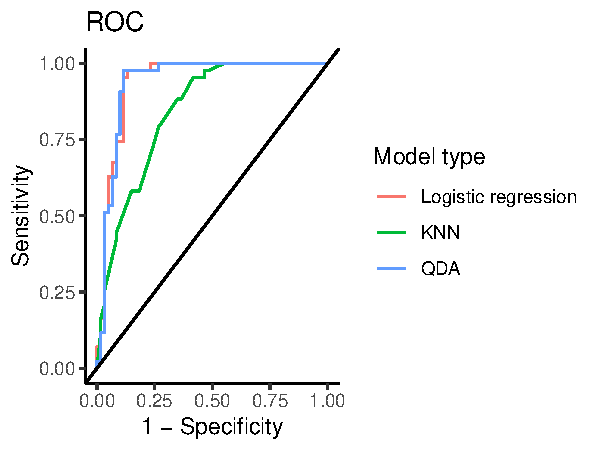
\includegraphics{hand-in_files/figure-latex/unnamed-chunk-9-1} \end{center}

\begin{Shaded}
\begin{Highlighting}[]
\CommentTok{\# AUC for the classifiers}
\NormalTok{roc.LR}\SpecialCharTok{$}\NormalTok{auc}
\end{Highlighting}
\end{Shaded}

\begin{verbatim}
## Area under the curve: 0.9391
\end{verbatim}

\begin{Shaded}
\begin{Highlighting}[]
\NormalTok{roc.KNN}\SpecialCharTok{$}\NormalTok{auc}
\end{Highlighting}
\end{Shaded}

\begin{verbatim}
## Area under the curve: 0.8417
\end{verbatim}

\begin{Shaded}
\begin{Highlighting}[]
\NormalTok{roc.QDA}\SpecialCharTok{$}\NormalTok{auc}
\end{Highlighting}
\end{Shaded}

\begin{verbatim}
## Area under the curve: 0.938
\end{verbatim}

\hypertarget{ii-1}{%
\section{ii)}\label{ii-1}}

The ROC curve shows how the binary classifiers are performing with a
varying threshold. The plot shows the true positive rate, or
sensitivity, against the true negative rate, or 1 - specificity. If a
classifier is on the black diagonal line it performs just as good as
guessing randomly and if it lays above the diagonal line it performs
better. This means that a classifier is better the further up in the
left corner its ROC curve are. In this case the logistic regression and
the QDA performs better than the KNN classifier.

The AUC, or area under the curve, is just the area under the ROC curve
and provides an aggregate measure of all classifiers for all thresholds.
As expected, the AUC for the logistic regression and the QDA are higher
than the one for the KNN indicating better performance.

\hypertarget{iii-1}{%
\section{iii)}\label{iii-1}}

We would say the logistic regression model is the most interpretable
model. This model provides easy to understand betas telling about the
realtionship between the body mass and flipper length and if the penguin
is Adelie or not. The two other models does not provide the same
information about the data.

\hypertarget{c-2}{%
\subsection{c)}\label{c-2}}

\begin{Shaded}
\begin{Highlighting}[]
\NormalTok{model.LR}\SpecialCharTok{$}\NormalTok{coefficients}
\end{Highlighting}
\end{Shaded}

\begin{verbatim}
##       (Intercept)       body_mass_g flipper_length_mm 
##        37.7618776         0.0007120        -0.2055804
\end{verbatim}

Increasing the body mass of penguin with 1000g will result in the
following change in the oddds

\$\$ \begin{equation}

exp(0.0007120 * 1000) = 2.028

\end{equation}

\$\$

The odds increases by a factor of 2.028.

\hypertarget{d-1}{%
\subsection{d)}\label{d-1}}

\begin{Shaded}
\begin{Highlighting}[]
\CommentTok{\# Get all data, from both test and training}
\NormalTok{penguins.pred.all }\OtherTok{\textless{}{-}}\NormalTok{ Penguins\_reduced }\SpecialCharTok{\%\textgreater{}\%}\NormalTok{ dplyr}\SpecialCharTok{::}\FunctionTok{select}\NormalTok{(}\SpecialCharTok{{-}}\NormalTok{adelie)}

\CommentTok{\# Classify on both test and training data using LR model}
\NormalTok{pred.all }\OtherTok{\textless{}{-}} \FunctionTok{ifelse}\NormalTok{(model.LR }\SpecialCharTok{\%\textgreater{}\%} \FunctionTok{predict}\NormalTok{(penguins.pred.all) }\SpecialCharTok{\textgreater{}} \FloatTok{0.5}\NormalTok{, }\DecValTok{1}\NormalTok{, }\DecValTok{0}\NormalTok{)}

\NormalTok{penguins.pred.all }\OtherTok{\textless{}{-}}\NormalTok{ Penguins\_reduced }\SpecialCharTok{\%\textgreater{}\%}\NormalTok{ dplyr}\SpecialCharTok{::}\FunctionTok{mutate}\NormalTok{(}\AttributeTok{pred =}\NormalTok{ pred.all)}

\CommentTok{\# Plot result}
\FunctionTok{ggplot}\NormalTok{(penguins.pred.all, }\FunctionTok{aes}\NormalTok{(}\AttributeTok{x=}\NormalTok{flipper\_length\_mm, }\AttributeTok{y=}\NormalTok{body\_mass\_g)) }\SpecialCharTok{+} 
  \FunctionTok{ggtitle}\NormalTok{(}\StringTok{"Classification of penguins"}\NormalTok{) }\SpecialCharTok{+}
  \FunctionTok{geom\_point}\NormalTok{(}\FunctionTok{aes}\NormalTok{(}\AttributeTok{col =} \FunctionTok{as.factor}\NormalTok{(adelie), }\AttributeTok{shape =} \FunctionTok{as.factor}\NormalTok{(pred))) }\SpecialCharTok{+} 
  \FunctionTok{labs}\NormalTok{(}\AttributeTok{x =} \StringTok{"Flipper length [mm]"}\NormalTok{,}
       \AttributeTok{y =} \StringTok{"Body mass [g]"}\NormalTok{,}
       \AttributeTok{col =} \StringTok{"True class"}\NormalTok{,}
       \AttributeTok{shape =} \StringTok{"Predicted class"}\NormalTok{) }\SpecialCharTok{+} 
  \FunctionTok{scale\_colour\_discrete}\NormalTok{(}\AttributeTok{labels=}\FunctionTok{c}\NormalTok{(}\StringTok{"Not Adelie"}\NormalTok{, }\StringTok{"Adelie"}\NormalTok{)) }\SpecialCharTok{+}
  \FunctionTok{scale\_shape\_discrete}\NormalTok{(}\AttributeTok{labels=}\FunctionTok{c}\NormalTok{(}\StringTok{"Not Adelie"}\NormalTok{, }\StringTok{"Adelie"}\NormalTok{))}
\end{Highlighting}
\end{Shaded}

\begin{center}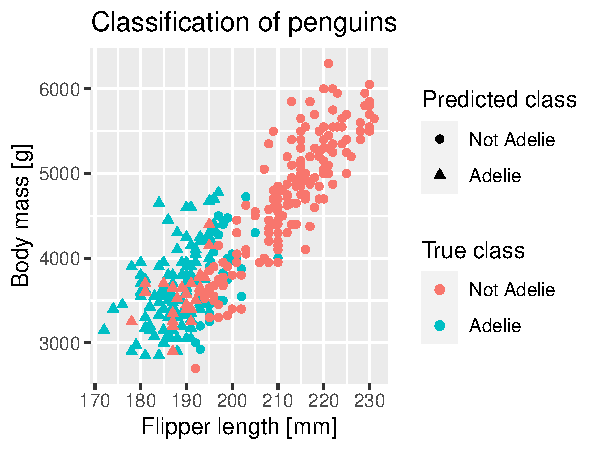
\includegraphics{hand-in_files/figure-latex/unnamed-chunk-11-1} \end{center}

\hypertarget{problem-4}{%
\section{Problem 4}\label{problem-4}}

\end{document}
